%%%%%%%%%%%%%%%%%%%%%%%%%%%%%%%%%%%%%%%%%%%%%%%%%%%%%%%%%%%%%%%%%%%%%%
\section{\label{sec:install}Installation}
%%%%%%%%%%%%%%%%%%%%%%%%%%%%%%%%%%%%%%%%%%%%%%%%%%%%%%%%%%%%%%%%%%%%%%

This section contains the instructions for installing Condor at your
Unix site.

There are two sets of instructions for installing Condor.
They are identified as the older and the newer installation
instructions.
All discussion prior to installation is valid whether using
the newer installation script or the older method.
The installation will have a default configuration that can
be customized.
Sections of the manual that follow this one explain customization.

Read this entire section before starting installation.

Please read the copyright and disclaimer information in 
section~\ref{sec:condor-public-license} on
page~\pageref{sec:condor-public-license} of the manual, or in the
file \File{LICENSE.TXT}, before proceeding.  Installation and
use of Condor is acknowledgment that you have read and agree to the
terms.

%%%%%%%%%%%%%%%%%%%%%%%%%%%%%%%%%%%%%%%%%%%%%%%%%%%%%%%%%%%%%%%%%%%%%%
\subsection{\label{sec:pre-install-procedure}
Obtaining Condor}
%%%%%%%%%%%%%%%%%%%%%%%%%%%%%%%%%%%%%%%%%%%%%%%%%%%%%%%%%%%%%%%%%%%%%%
\index{installation!download}
\index{Unix installation!download}
\index{download}
The first step to installing Condor is to download it from the Condor
web site, \URL{http://www.cs.wisc.edu/condor}.
The downloads are available from the downloads page,
at \URL{http://www.cs.wisc.edu/condor/downloads/}.

The platform-dependent Condor files are currently available from two sites.
The main site is at the University of Wisconsin--Madison,
Madison, Wisconsin, USA.
A second site is the Istituto Nazionale di Fisica Nucleare Sezione di
Bologna, Bologna, Italy.
Please choose the site nearest to you.

Make note of the location of where you download the binary into.

The Condor binary distribution is packaged in the following 5 files
and 2 directories:

\begin{description}
\item[\File{DOC}] directions on where to find Condor documentation
\item[\File{INSTALL}] these installation directions
\item[\File{LICENSE.TXT}] the licensing agreement.
                  By installing Condor, you agree to the contents of
		  this file
\item[\File{README}] general information
\item[\File{condor\_install}] the Perl script used to install and
                  configure Condor
\item[\File{examples}] directory containing C, Fortran and C++ example
		  programs to run with Condor
\item[\File{release.tar}] tar file of the release directory, which contains
		  the Condor binaries and libraries
\end{description}

Before you install, please consider joining the condor-world mailing
list.
Traffic on this list is kept to an absolute minimum.
It is only used to announce new releases of Condor.
To subscribe, send a message to \Email{majordomo@cs.wisc.edu} with the body:
\begin{verbatim}
   subscribe condor-world 
\end{verbatim}

%%%%%%%%%%%%%%%%%%%%%%%%%%%%%%%%%%%%%%%%%%%%%%%%%%%%%%%%%%%%%%%%%%%%%%
\subsection{\label{sec:Preparing-to-Install}Preparation} 
%%%%%%%%%%%%%%%%%%%%%%%%%%%%%%%%%%%%%%%%%%%%%%%%%%%%%%%%%%%%%%%%%%%%%%

Before installation, make a few important
decisions about the basic layout of your pool.
The decisions answer the questions:

\begin{enumerate}
\item What machine will be the central manager?
\item What machines should be allowed to submit jobs?
\item Will Condor run as root or not?
\item Who will be administering Condor on the machines in your pool?
\item Will you have a Unix user named condor and will its home directory be
   shared? 
\item Where should the machine-specific directories for Condor go?
\item Where should the parts of the Condor system be installed? 
	\begin{itemize}
	\item Configuration files
	\item Release directory
		\begin{itemize}
		\item user binaries
		\item system binaries 
		\item \File{lib} directory
	  	\item \File{etc} directory
		\end{itemize}
	\item Documentation
	\end{itemize}
\item Am I using AFS?
\item Do I have enough disk space for Condor?
\end{enumerate}

\begin{description}

\item[1. What machine will be the central manager?]

One machine in your pool must be the central manager.
\index{central manager!installation issues}
Install Condor on this machine first.
This is the centralized information repository for the Condor pool,
and it is also the
machine that does match-making between available machines and
submitted jobs.
If the central manager machine crashes, any currently active
matches in the system will keep running, but no new matches will be
made.  Moreover, most Condor tools will stop working.  Because of the
importance of this machine for the proper functioning of Condor,
install the central manager on a machine that is likely to stay up all the
time, or on one that will be rebooted quickly if it does crash.

Also consider
network traffic and your network layout when choosing your central
manager.
All the daemons send updates (by default, every 5 minutes) to this machine.
Memory requirements for the central manager differ by the number of machines
in the pool.
A pool with up to about 100 machines will require approximately
25 Mbytes of memory for the central manager's tasks.
A pool with about 1000 machines will require approximately
100 Mbytes of memory for the central manager's tasks.

A faster CPU will improve the time to do matchmaking. 

\item[2. Which machines should be allowed to submit jobs?]

Condor can restrict the machines allowed to submit jobs.  Alternatively, 
it can allow any machine the network allows to connect to a submit machine
to submit jobs.  If the Condor pool is behind a firewall, and all machines
inside the firewall are trusted, the \Macro{HOSTALLOW\_WRITE} configuration
entry can be set to *.  Otherwise, it should be set to reflect
the set of machines permitted to submit jobs to this pool.
Condor tries to be secure by default,
so out of the box, the configuration file ships with an invalid definition
for this configuration variable.
This invalid value allows no machine to connect and submit
jobs, so after installation, change this entry.
Look for the
entry defined with the value
\Expr{YOU\_MUST\_CHANGE\_THIS\_INVALID\_CONDOR\_CONFIGURATION\_VALUE}.

\item[3. Will Condor run as root or not?]

\index{installation!running as root}
Start up the Condor daemons as the Unix user root.
Without this,
Condor can do very little to enforce security and policy
decisions.
You can install Condor as any user,
however there are both serious security and performance consequences.
Please see section~\ref{sec:Non-Root} on page~\pageref{sec:Non-Root}
in the manual for the details and ramifications of
running Condor as a Unix user other than root.

\item[4. Who will administer Condor?]

\index{Condor!Unix administrator}
\index{Unix administrator}
\index{Unix user!root}

% administrator is a person, not an account
% responsibilities of the administrator needed here
% 1. to install
% 2. to customize policies
% 3. to receive e-mail

Either root will be administering Condor directly, or someone else
would be acting as the Condor administrator.  If root has delegated
the responsibility to another person but doesn't want to grant that
person root access, root can specify a 
\File{condor\_config.root} file that
will override settings in the other condor configuration
files.  This way,
the global 
\File{condor\_config} file can be owned and controlled by whoever
is condor-admin, and the 
condor\_config.root can be owned and
controlled only by root.  Settings that would compromise root security
(such as which binaries are started as root) can be specified in the
\File{condor\_config.root} file while other settings that only control policy
or condor-specific settings can still be controlled without root
access.  


\item[5. Will you have a Unix user named condor, and will its home
directory be shared?]

\index{Unix user!condor}
To simplify installation of Condor,
create a Unix user named condor on all machines in the pool.
The Condor daemons will create files
(such as the log files) owned by this user,
and the home directory can be used to specify the location of files
and directories needed by Condor.  The home directory of this user can
either be shared among all machines in your pool, or could be a
separate home directory on the local partition of each machine.  Both
approaches have advantages and disadvantages.  Having the directories
centralized can make administration easier, but also concentrates the
resource usage such that you potentially need a lot of space for a
single shared home directory.  See the section below on
machine-specific directories for more details.

If you choose not to create a user named condor,
then you must specify either via the
\index{environment variables!CONDOR\_IDS@\texttt{CONDOR\_IDS}}
\index{CONDOR\_IDS@\texttt{CONDOR\_IDS}!environment variable}
\Env{CONDOR\_IDS} environment variable or the \Macro{CONDOR\_IDS}
config file setting which uid.gid pair should be used for
the ownership of various Condor files.  
See section~\ref{sec:uids} on UIDs in Condor on
page~\pageref{sec:uids} in the Administrator's Manual for details.

\item[6. Where should the machine-specific directories for
Condor go?]

Condor needs a few directories that are unique on every machine in
your pool.  These are 
\File{spool}, 
\File{log}, and 
\File{execute}.  Generally, all
three are subdirectories of a single machine specific directory called
the local directory (specified by the \Macro{LOCAL\_DIR} macro
in the configuration file).
Each should be owned by the user that Condor is to be run as.
\index{owner!of directories}

If you have a Unix user named condor with a local home directory on each
machine, the \MacroNI{LOCAL\_DIR} could just be user condor's home
directory (\MacroNI{LOCAL\_DIR} = \MacroUNI{TILDE} in the 
configuration file).
If this user's home directory is shared among all machines in your
pool, you would want to create a directory for each host (named by
host name) for the local directory (for example, \MacroNI{LOCAL\_DIR} =
\MacroUNI{TILDE}/hosts/\MacroUNI{HOSTNAME}).  If you do not
have a condor account on your machines, you can put these directories
wherever you'd like.
However, where to place them will require some
thought, as each one has its own resource needs:

\begin{description}
\index{Unix directory!\File{execute}}
\index{disk space requirement!\File{execute} directory}
\item[\File{execute}] This is the directory that acts as the current working
directory for any Condor jobs that run on a given execute machine.
The binary for the remote job is copied into this directory, so
there
must be enough space for it.  (Condor will not send a job to a
machine that does not have enough disk space to hold the initial
binary).  In addition, if the remote job dumps core for some reason,
it is first dumped to the execute directory before it is sent back to
the submit machine.  So, put the execute directory on
a partition with enough space to hold a possible core file from the
jobs submitted to your pool.

\index{Unix directory!\File{spool}}
\index{disk space requirement!\File{spool} directory}
\item[\File{spool}] The \File{spool} directory holds the job queue
and history files,
and the checkpoint files for all jobs submitted from a given machine.
As a result, disk space requirements for the \File{spool} directory
can be quite large,
particularly if users are submitting jobs with very large
executables or image sizes.
By using a checkpoint server
(see section~\ref{sec:Ckpt-Server} on Installing a Checkpoint Server on
page~\pageref{sec:Ckpt-Server} for details),
you can ease the disk
space requirements, since all checkpoint files are stored on the
server instead of the spool directories for each machine.  However,
the initial checkpoint files (the executables for all the clusters you
submit) are still stored in the spool directory, so you will need
%
% how much?!?
%
some space, even with a checkpoint server.

\index{Unix directory!\File{log}}
\index{disk space requirement!\File{log} directory}
\item[\File{log}] Each Condor daemon writes its own log file,
and each log file is placed
in the \File{log} directory.  You can specify what size you want these files
to grow to before they are rotated,
%
% rotated?  Maybe this is talking about wrapping around to
% overwrite the oldest entries first
%
so the disk space requirements of
the directory are configurable.
The larger the log files, the more
historical information they will hold if there is a problem, but the
more disk space they use up.  If you have a network file system
installed at your pool, you might want to place the log directories in
a shared location (such as \File{/usr/local/condor/logs/\$(HOSTNAME)}),
so that you can view the log files from all your machines in a single
location.  However, if you take this approach, you will have to
specify a local partition for the \File{lock} directory (see below).

\index{Unix directory!\File{lock}}
\item[lock] Condor uses a small number of lock files to synchronize
access to certain files that are shared between multiple daemons.
Because of problems encountered with file locking and network
file systems (particularly NFS), these lock files should be placed on a
local partition on each machine.  By default, they are placed in
the \File{log} directory.  If you place your \File{log}
directory on a network file system partition,
specify a local partition for the
lock files with the \Macro{LOCK} parameter in the configuration file (such as
\File{/var/lock/condor}).

\end{description}

\index{disk space requirement!Condor files}
Generally speaking, it is recommended that you do not put these directories
(except \File{lock}) on the same partition as \File{/var},
since if the partition
fills up, you will fill up \File{/var} as well. 
This will cause lots of
problems for your machines.  Ideally, you will have a separate partition
for the Condor directories. Then, the only consequence of filling up
the directories
will be Condor's malfunction, not your whole machine.

\item[7. Where should the parts of the Condor system be installed?]

	\begin{itemize}
	\item Configuration Files
	\item Release directory
		\begin{itemize}
		\item User Binaries
		\item System Binaries 
		\item \File{lib} Directory
	  	\item \File{etc} Directory
		\end{itemize}
	\item Documentation
	\end{itemize}

\begin{description}
\item[Configuration Files] There are a number of configuration files
that allow you
different levels of control over how Condor is configured at each
machine in your pool.  
The global configuration file is shared by all machines in the pool.
For ease of administration, this file should be located on a shared
file system, if possible.
In addition, there is a local
configuration file for each machine, where you can override settings in the
global file.  This allows you to have different daemons running,
different policies for when to start and stop Condor jobs, and so on.
You can also have configuration files specific to each platform in your pool.
See
section~\ref{sec:Multiple-Platforms} on
page~\pageref{sec:Multiple-Platforms} about Configuring Condor for
Multiple Platforms for details.

In addition, because we recommend that you start the Condor daemons as
root, we allow you to create configuration files that are owned and
controlled by root that will override any other Condor settings.  This
way, if the Condor administrator is not root, the regular Condor configuration
files can be owned and writable by condor-admin, but root does not have
to grant root access to this person.  See
section~\ref{Root-Config} on page~\pageref{Root-Config} in the
manual for a detailed discussion of the root configuration files, if you
should use them, and what settings should be in them.

\index{configuration files!location}
In general, there are a number of places that Condor will look to find
its configuration files.  The first file it looks for is the global configuration
file.  These locations are searched in order until a configuration file is
found.  If none contain a valid configuration file, Condor will print an
error message and exit:
\begin{enumerate}
   \item File specified in the \Env{CONDOR\_CONFIG} environment variable
   \item \File{/etc/condor/condor\_config}
   \item \File{\Tilde condor/condor\_config}
   \item \File{\$(GLOBUS\_LOCATION)/etc/condor\_config}
\end{enumerate}

If you specify a file in the \Env{CONDOR\_CONFIG} environment variable
and there's a problem reading that file, Condor will print an error
message and exit right away, instead of continuing to search the other
options.
However, if no \Env{CONDOR\_CONFIG} environment variable is set,
Condor will search through the other options.

Next, Condor tries to load the local configuration file(s).
The only way to specify the local configuration file(s) is in the global configuration
file, with the \Macro{LOCAL\_CONFIG\_FILE} macro.  If that macro is not
set, no local configuration file is used.  This macro can be a list of files
or a single file.

The root configuration files come in last.  The global file is searched for
in the following places:
\begin{enumerate}
   \item \File{/etc/condor/condor\_config.root}
   \item \File{\Tilde condor/condor\_config.root}
\end{enumerate}

The local root configuration file(s) are found with the
\Macro{LOCAL\_ROOT\_CONFIG\_FILE} macro.  If that is not set, no local
root configuration file is used.  This
macro can be a list of files or a single file.

\item[Release Directory]

Every binary distribution contains a \File{release.tar} file that contains
five subdirectories: \File{bin}, \File{etc}, \File{lib}, \File{sbin},
and \File{libexec}. Wherever you
choose to install these five directories we call the release directory
(specified by the \Macro{RELEASE\_DIR} macro in the configuration file).
Each
release directory contains platform-dependent binaries and libraries,
so you will need to install a separate one for each kind of machine in
your pool.  For ease of administration, these directories should be
located on a shared file system, if possible.

\begin{itemize}
     \item User Binaries:

     All of the files in the \File{bin} directory are programs the end
     Condor users should expect to have in their path.  You could
     either put them in a well known location (such as
     \File{/usr/local/condor/bin}) which you have Condor users add to
     their \Env{PATH} environment variable, or copy those files
     directly into a well known place already in the user's PATHs (such as
     \File{/usr/local/bin}).  With the above examples, you could also
     leave the binaries in \File{/usr/local/condor/bin} and put in
     soft links from \File{/usr/local/bin} to point to each program.

     \item System Binaries:

     All of the files in the \File{sbin} directory are Condor daemons and
     agents, or programs that only the Condor administrator would need
     to run.  Therefore, add these programs only
     to the \Env{PATH} of the Condor administrator.

     \item Private Condor Binaries:

     All of the files in the \File{libexec} directory are Condor
     programs that should never be run by hand, but are only used
     internally by Condor. 

     \item \File{lib} Directory:

     The files in the \File{lib} directory are the Condor libraries that
     must be linked in with user jobs for all of Condor's
     checkpointing and migration features to be used.  \File{lib} also
     contains scripts used by the \Condor{compile} program to help
     re-link jobs with the Condor libraries.  These files should be
     placed in a location that is world-readable, but they do not need
     to be placed in anyone's \Env{PATH}.  The \Condor{compile} script checks
     the configuration file for the location of the \File{lib} directory.

     \item \File{etc} Directory:

     \File{etc} contains an \File{examples} subdirectory which holds various
     example configuration files and other files used for installing Condor.
     \File{etc} is the recommended location to keep the master copy of your
     configuration files.  You can put in soft links from one of the places
     mentioned above that Condor checks automatically to find its
     global configuration file. 
\end{itemize}

\item[Documentation]

The documentation provided with Condor is currently available in
     HTML, Postscript and PDF (Adobe Acrobat).  It can be locally installed
     wherever is customary at your site.  You can also find the Condor
     documentation on the web at:
     \URL{http://www.cs.wisc.edu/condor/manual}.

\end{description}

\item[7. Am I using AFS?]

If you are using AFS at your site, be sure to read the
section~\ref{sec:Condor-AFS} on page~\pageref{sec:Condor-AFS} in the
manual.
Condor does not currently have a way to authenticate itself to AFS.
A solution is not ready for
\VersionNotice.
This implies that you are probably not going to want
to have the \Macro{LOCAL\_DIR} for Condor on AFS.
However, you can
(and probably should) have the Condor \MacroNI{RELEASE\_DIR} on AFS, so
that you can share one copy of those files and upgrade them in a
centralized location.  You will also have to do something special if
you submit jobs to Condor from a directory on AFS.  Again, read manual
section~\ref{sec:Condor-AFS} for all the details.

\item[8. Do I have enough disk space for Condor?]

\index{disk space requirement!all versions}
Condor takes up a fair amount of space.
This is another reason why it is a good idea to have it on a shared
file system.
The size requirements for the downloads are given on the
downloads page.
They currently vary from about 20 Mbytes (statically linked HP Unix
on a PA RISC)
to more than 50 Mbytes (dynamically linked Irix on an SGI).

%listed in table~\ref{install-sizes}.

%\begin{center}
%\begin{table}
%\begin{tabular}{|ll|} \hline
%\emph{Platform} 	&	\emph{Size}		\\	\hline \hline
%         Intel/Linux   &	11   Mbytes (statically linked) \\
%         Intel/Linux   &	6.5 Mbytes (dynamically linked) \\
%         Intel/Solaris &	8   Mbytes \\
%         Sparc/Solaris &	10   Mbytes \\
%         Alpha/Digital Unix & 	15.5 Mbytes \\ \hline
%\end{tabular}
%\caption{\label{install-sizes}Release Directory Size Requirements}
%\end{table}
%\end{center}

In addition, you will need a lot of disk space in the local directory
of any machines that are submitting jobs to Condor.  See question 6
above for details on this.

\end{description}

%%%%%%%%%%%%%%%%%%%%%%%%%%%%%%%%%%%%%%%%%%%%%%%%%%%%%%%%%%%%%%%%%%%%%%
\subsection{\label{sec:new-install-procedure}
Newer Unix Installation Procedure}
%%%%%%%%%%%%%%%%%%%%%%%%%%%%%%%%%%%%%%%%%%%%%%%%%%%%%%%%%%%%%%%%%%%%%%

\index{installation!with \Condor{configure}}
\index{condor\_configure@\Condor{configure}}
The Perl script \Condor{configure} installs Condor.
Command-line arguments specify all needed information to this
script.  The script can be executed multiple times, to modify or further
set the configuration.  \Condor{configure} has been tested using Perl 5.003.
Use this or a more recent version of Perl.

After download, all the files are in a compressed, tar format.
They need to be untarred, as
\begin{verbatim}
  tar xzf completename.tar.gz
\end{verbatim}
After untarring, the directory will have the Perl script
\Condor{configure}, as well as a second tar file called
\File{release.tar}.
\Condor{configure} works on \File{release.tar}.

\Condor{configure} is completely command-line driven; it is not interactive.
Several command-line arguments are always needed with \Condor{configure}.
The argument
\begin{verbatim}
  --install=/path/to/release.tar
\end{verbatim}
specifies the path to the Condor release tarball. 
The argument
\begin{verbatim}
--install-dir=directory
\end{verbatim}
specifies the path to the install directory.
The argument
\begin{verbatim}
--local-dir=directory
\end{verbatim}
specifies the path to the local directory.

The \Opt{--type} option to \Condor{configure}
specifies one or more of the roles that a machine may take on
within the Condor pool: central manager, submit or execute.
These options are given in a comma separated list.
So, if a machine is both a submit and execute
machine, 
the proper command-line option is
\begin{verbatim}
--type=manager,execute
\end{verbatim}

Configure Condor on the central manager machine first.  If Condor
will run as root in this pool (Item 3 above), run \Condor{configure} 
as root, and it will install and set the file permissions correctly.  
On the central manager machine, run \Condor{configure} as follows.
\begin{verbatim}
% condor_configure --install=r.tar --install-dir=~condor \
	--local-dir=/scratch/condor --type=manager
\end{verbatim}

The central manager can also be a submit point or and execute machine, but
this is only recommended for very small pools.
If this is the case, the \Opt{--type} option changes to
\Expr{manager,execute} or \Expr{manager,submit}  or 
\Expr{manager,submit,execute}.

After the central manager is installed, the execute and submit machines
should then be configured.  Decisions about whether to run Condor as root
should be consistent throughout the pool. For each machine in the pool,
run

\begin{verbatim}
% condor_configure --install=r.tar --install-dir=~condor \
	--local-dir=/scratch/condor --type=execute,submit
\end{verbatim}

See the \Condor{configure} manual page in
section~\ref{man-condor-configure} on
page~\pageref{man-condor-configure} for details.

Please skip to section~\ref{installed-now-what} for final instructions
on configuring and starting Condor.

%%%%%%%%%%%%%%%%%%%%%%%%%%%%%%%%%%%%%%%%%%%%%%%%%%%%%%%%%%%%%%%%%%%%%%
\subsection{\label{sec:install-procedure}
Older Unix Installation Procedure}
%%%%%%%%%%%%%%%%%%%%%%%%%%%%%%%%%%%%%%%%%%%%%%%%%%%%%%%%%%%%%%%%%%%%%%

IF YOU HAVE DECIDED TO CREATE A condor USER AND GROUP, DO
THAT ON ALL YOUR MACHINES BEFORE YOU DO ANYTHING ELSE.

After download, all the files are in a compressed, tar format.
They need to be untarred, as
\begin{verbatim}
        tar xzf completename.tar.gz
\end{verbatim}

\index{installation!scripts}
\index{Unix installation!scripts}
To install Condor, use one or both of the scripts
provided to help you: \Condor{install} and \Condor{init}.
\index{condor\_install script@\Condor{install} script}
\index{condor\_init script@\Condor{init} script}
Run these scripts as the user that you are going to run the Condor
daemons as.  First, run \Condor{install} on the machine that will be a
file server for shared files used by Condor, such as the release
directory, and possibly the condor user's home directory.  When you
do, choose the ``full-install'' option in step \#1 described below.

Once you have run \Condor{install} on a file server to set up your
release directory and configure Condor for your site, you should run
\Condor{init} on any other machines in your pool to create any locally
used files that are not created by \Condor{install}.  In the most
simple case, where nearly all of Condor is installed on a shared file
system, even though \Condor{install} will create nearly all the files
and directories you need, you will still need to use \Condor{init} to
create the \Macro{LOCK} directory on the local disk of each machine.
If you have a shared release directory, but the \MacroNI{LOCAL\_DIR} is
local on each machine, \Condor{init} will create all the directories
and files needed in \MacroNI{LOCAL\_DIR}.  In addition, \Condor{init}
will create any soft links on each machine that are needed so that
Condor can find its global configuration file.

If you do not have a shared file system, you need to run
\Condor{install} on each machine in your pool to set up Condor.  In
this case, there is no need to run \Condor{init} at all.

In addition, you will want to run \Condor{install} on your central
manager machine if that machine is different from your file server,
using the ``central-manager'' option in step \#1 described below.  Run
\Condor{install} on your file server first, then on your central
manager.  If this step fails for some reason (NFS permissions, etc),
you can do it manually quite easily.  All this does is copy the
\File{condor\_config.local.central.manager} file from
\Release{etc/examples} to the proper location for the local configuration
file of your central manager machine.  If your central manager is an
Alpha or an SGI, you might want to add \Macro{KBDD} to the
\MacroU{DAEMON\_LIST} macro.  See
section~\ref{sec:Configuring-Condor} Configuring Condor on
page~\pageref{sec:Configuring-Condor} of the manual for details.

\Condor{install} assumes you have perl installed in \File{/usr/bin/perl}.  If
this is not the case, you can either edit the script to put in the right
path, or you will have to invoke perl directly from your shell
(assuming perl is in your PATH):
\begin{verbatim}
% perl condor_install
\end{verbatim}

\Condor{install} breaks down the installation procedure into various
steps.  Each step is clearly numbered.  The following section explains
what each step is for, and suggests how to answer the questions
\Condor{install} will ask you for each one.

%%%%%%%%%%%%%%%%%%%%%%%%%%%%%%%%%%%%%%%%%%%%%%%%%%%%%%%%%%%%%%%%%%%%%%
\subsubsection{\Condor{install}, step-by-step}
%%%%%%%%%%%%%%%%%%%%%%%%%%%%%%%%%%%%%%%%%%%%%%%%%%%%%%%%%%%%%%%%%%%%%%

\begin{description}
\item[STEP 1: What type of Condor installation do you want?]

     There are three types of Condor installation you might choose:
     'submit-only', 'full-install', and 'central-manager'.  A
     submit-only machine can submit jobs to a Condor pool, but Condor
     jobs will not run on it.  A full-install machine can both submit
     and run Condor jobs.  

     If you are planning to run Condor jobs on your machines, you
     should either install and run Condor as root, or as the Unix
     user condor.  

     If you are planning to set up a submit-only machine, you can
     either install Condor machine-wide as root or user condor, or,
     you can install Condor as yourself into your home directory.

     The other possible installation type is setting up a machine as a
     central manager.  If you do a full-install and you say that you
     want the local host to be your central manager, this step will be
     done automatically.  You should only choose the central-manager
     option at step 1 if you have already run \Condor{install} on your
     file server and you now want to run \Condor{install} on a different
     machine that will be your central manager.

\item[STEP 2: How many machines are you setting up this way?]

     If you are installing Condor for multiple machines and you have
     a shared file system, then \Condor{install} will prompt you for the
     host names of each machine you want to add to your Condor pool.
     If you do not have a shared file system, you will have to run
     \Condor{install} locally on each machine, so \Condor{install}
     does not
     ask for the names.  If you provide a list, it will
     use the names to automatically create directories and files
     later.  At the end, \Condor{install} will dump out this list to a
     \File{roster} file which can be used by scripts to help maintain your
     Condor pool.

     If you are only installing Condor on 1 machine, you would
     answer no to the first question, and move on.

\item[STEP 3: Install the Condor release directory] 
     The release directory contains five subdirectories: 
     \File{bin}, \File{etc},
     \File{lib}, \File{libexec} and \File{sbin}.  
     \File{bin} contains user-level executable programs.
     \File{etc} is the recommended location for your Condor configuration
     files, and
     it also includes an \File{examples} directory with default
     configuration files
     and other default files used for installing Condor.  \File{lib} contains
     libraries to link Condor user programs and scripts used by the
     Condor system.  \File{sbin} contains all administrative executable
     programs and the Condor daemons.  \File{libexec} contains
     programs that only Condor needs to execute.

     If you have multiple machines with a shared file system that will
     be running Condor, put the release directory on that
     shared file system so you only have one copy of all the binaries,
     and so that when you update them, you can do so in one place.
     Note that the release directory is architecture dependent, so
     download separate binary distributions for every
     platform in your pool.

     \Condor{install} tries to find an already installed release
     directory.  If it cannot find one, it asks if you have installed
     one already.  If you have not installed one, it tries to do so
     for you by untarring the \File{release.tar} file from the binary
     distribution.  

\Note If you are only setting up a central manager (you chose 'central
     manager' in STEP 1), STEP 3 is the last question you will need to
     answer.

\item[STEP 4: How and where should Condor send e-mail if things go wrong?]

\index{administrator!e-mail to}
     Various parts of Condor will send e-mail to a condor administrator
     if something goes wrong that needs human attention.  You will
     need to specify the e-mail address of this administrator.  

     You also specify the full path to a mail program
     that Condor will use to send the e-mail.  This program needs to
     understand the \Opt{-s} option, to specify a subject
     for the outgoing message.  The default on most platforms will
     probably be correct.  On Linux machines, since there is such
     variation in Linux distributions and installations,
     verify that the default works.  If the script complains that it
     cannot find the mail program that was specified, try
\begin{verbatim}
% which mail
\end{verbatim}
     to see what mail program is
     currently in your PATH.  If there is none, try 
\begin{verbatim}
% which mailx
\end{verbatim}
     If you still cannot find anything, ask your system administrator.
     Verify that the program you use supports
     \Opt{-s}.  The man page for that program will probably tell you.

\item[STEP 5: File system and UID domains.]

     Condor does not depend on a shared file system and common UID
     space for running jobs outside the standard universe.
     Jobs can specify file transfer within the submit description file.
     See
     section~\ref{sec:file-transfer} on page~\pageref{sec:file-transfer}
     for information on properly setting up file transfer for jobs.

     To utilize the convenience of a shared file system (such as NFS),
     a common UID space is needed.  
     This is one in which there is a unique mapping of user names to
     UIDs across all machines in the common UID space.
     It is important to correctly configure
     Condor with respect to a shared file system.
     For complete details on what these settings do and how you
     should answer the questions, read
     section~\ref{sec:Shared-Filesystem-Config-File-Entries},
     Shared File System Configuration File Entries'', on
     page~\pageref{sec:Shared-Filesystem-Config-File-Entries}.

     You will be asked if you have a shared file system.  If so,
     \condor{install} will configure your \Macro{FILESYSTEM\_DOMAIN} 
     setting to be set to the domain name of the machine running
     \condor{install}.
     If not, \MacroNI{FILESYSTEM\_DOMAIN} will be set to
     \MacroUNI{FULL\_HOSTNAME}, indicating that each machine is in its
     own domain.

     For the UID domain, Condor needs to know if all user names across all
     the machines in the pool have a unique UID.  
     If so, \Macro{UID\_DOMAIN} will be set to the domain name of the
     machine running \condor{install}. 
     If not, \MacroNI{UID\_DOMAIN} will be set to
     \MacroUNI{FULL\_HOSTNAME}, indicating that each machine is in its 
     own domain.

     If you have a common \MacroNI{UID\_DOMAIN}, \condor{install} will
     ask if you have a \Term{soft UID domain}, meaning that although
     you have unique UIDs, not every machine in your pool has all the
     users in their individual password files.  Please see the
     description of \Macro{SOFT\_UID\_DOMAIN} in
     section~\ref{param:SoftUidDomain} on
     page~\pageref{param:SoftUidDomain} for details.  

\item[STEP 6: Java Universe support in Condor.]

	Condor has the ability to run Java programs with remote i/o,
	but no checkpointing. If you would like to enable this feature
	in Condor, then select yes for enabling of Java Universe. The
	installer will try to determine if you have a valid JVM and
	prompt you if nothing suitable can be found. If you do not care
	to use the Java Universe, then it is safe to say no here.

\item[STEP 7: Where should public programs be installed?]

     It is recommended that you install the user-level Condor programs
     in the release directory, (where they go by default).  This way,
     when you want to install a new version of the Condor binaries,
     you can just replace your release directory and everything will
     be updated at once.  So, one option is to have Condor users add
     \Release{bin} to their PATH, so that they can access the
     programs.  However, we recommend putting in soft links from some
     directory already in their PATH (such as \File{/usr/local/bin}) that
     point back to the Condor user programs.  \Condor{install} will do
     this for you. All you do is tell it what directory to put
     these links into.  This way, users do not have to change their
     PATH to use Condor, and you can still have the binaries installed
     in their own location.

% untwist this first sentence!
     If you are installing Condor as neither root nor condor, there is
     a perl script wrapper to all the Condor tools that is created
     which sets some appropriate environment variables and
     automatically passes certain options to the tools.  This is all
     created automatically by \Condor{install}.  So, you need to tell
     \Condor{install} where to put this perl script.  The script itself
     is linked to itself with many different names, since it is the
     name that determines the behavior of the script.  This script
     should go somewhere that is in your PATH already, if possible
     (such as \Tilde bin).

\end{description}

At this point, the remaining steps differ based on the
whether the installation is a full install or a submit-only.
Skip to the appropriate section below, based on the kind of installation.

%%%%%%%%%%%%%%%%%%%%%%%%%%%%%%%%%%%%%%%%%%%%%%%%%%%%%%%%%%%%%%%%%%%%%%
\subsubsection{Full Install}
%%%%%%%%%%%%%%%%%%%%%%%%%%%%%%%%%%%%%%%%%%%%%%%%%%%%%%%%%%%%%%%%%%%%%%

\begin{description}

\item[STEP 8: What machine will be your central manager?]

     Type in the full host name of the machine you have chosen
     for your central manager.  If \Condor{install} cannot find
     information about the host you typed by querying your name server,
     it will print out an error message and ask you to confirm.


\item[STEP 9: Where will the local directory go?]

     This is the directory discussed in question 5 of the installation
     introduction.  \Condor{install} tries to make some educated guesses
     as to what directory you want to use for the purpose.
     Agree to the correct guess, or (when \Condor{install} has run out
     of guesses) type in what you want.  Since this directory needs to
     be unique, it is common to use the host name of each machine in
     its name.  When typing in your own path, you can use
     '\MacroUNI{HOSTNAME}' which \Condor{install}
     (and the Condor configuration files)
     will expand to the host name of the machine you are currently on.
     \Condor{install} will try to create the corresponding directories
     for all the machines you told it about in STEP 2 above.

     Once you have selected the local directory, \Condor{install}
     creates all the needed subdirectories of each one with the proper
     permissions.  They should have the following permissions and
     ownerships:
\begin{verbatim}
     drwxr-xr-x   2 condor   root         1024 Mar  6 01:30 execute/
     drwxr-xr-x   2 condor   root         1024 Mar  6 01:30 log/
     drwxr-xr-x   2 condor   root         1024 Mar  6 01:30 spool/
\end{verbatim}

     If your local directory is on a shared file system,
     \Condor{install} will prompt you for the location of your lock
     files, as discussed in question \#5 above.  In this case, when
     \Condor{install} is finished, you will have to run \Condor{init} on
     each machine in your pool to create the \File{lock} directory before you
     can start up Condor.


\item[STEP 10: Where will the local (machine-specific) configuration files go?]

\index{configuration files!location}
     As discussed in question STEP 6 above, there are a few different
     levels of Condor configuration files.  There is the
     global configuration file
     that will be installed in \Release{etc/condor\_config}, and
     there are machine-specific, or local configuration files,
     that override
     the settings in the global file.  If you are installing on
     multiple machines or are configuring your central manager
     machine, you must select a location for your local 
     configuration files. 

     The two main options are to have a single directory that holds
     all the local configuration files, each one 
     named \File{\MacroUNI{HOSTNAME}.local},
     or to have the local configuration files go into the individual local
     directories for each machine.  Given a shared file system, we
     recommend the first option, since it makes it easier to configure
     your pool from a centralized location.


\item[STEP 11: How shall Condor find its configuration file?]

     Since there are a few known places Condor looks to find your
     configuration file, we recommend that you put a soft link from one of
     them to point to \Release{etc/condor\_config}.  This way, you
     can keep your Condor configuration in a centralized location, but
     all the Condor daemons and tools will be able to find their
     configuration files.  Alternatively, you can set the CONDOR\_CONFIG
     environment variable to contain \Release{etc/condor\_config}.

     \Condor{install} will ask you if you want to create a soft link
     from either of the two fixed locations that Condor searches.

\end{description}

Once you have completed STEP 11, you are done.  \Condor{install} prints
out a messages describing what to do next.  Please skip to 
section~\ref{installed-now-what}.

%%%%%%%%%%%%%%%%%%%%%%%%%%%%%%%%%%%%%%%%%%%%%%%%%%%%%%%%%%%%%%%%%%%%%%
\subsubsection{\label{Install-Submit-Only}
Submit Only}
%%%%%%%%%%%%%%%%%%%%%%%%%%%%%%%%%%%%%%%%%%%%%%%%%%%%%%%%%%%%%%%%%%%%%%

\index{submit-only installation}
\index{Unix installation!submit-only}
A submit-only installation of Condor implies that the machine will
be submitting jobs to one or more established Condor pools.
Configuration for this installation needs to account for the
other pools.

For the submit-only installation, STEP 6 continues and completes
the installation.

\begin{description}

\item[STEP 6: continued. ]
     A submit-only machine has the option of submission to more than
     one Condor pool.
     The full host name of the central manager is required for each
     pool.
     The first entered becomes the default for start up and job
     submission.

     There is a separate configuration file for each pool.
     The location of each file is specified.

     Identification of each pool requires a unique name. 
     A final question sets a name for each pool.
     The name will be the argument for \Opt{-pool} command line options.

\end{description}

%%%%%%%%%%%%%%%%%%%%%%%%%%%%%%%%%%%%%%%%%%%%%%%%%%%%%%%%%%%%%%%%%%%%%%
\subsection{\label{sec:install-rpms} RPMs}
%%%%%%%%%%%%%%%%%%%%%%%%%%%%%%%%%%%%%%%%%%%%%%%%%%%%%%%%%%%%%%%%%%%%%%

\index{installation!using Linux RPMs}
\index{RPM installation on Linux}
RPMs are available in \VersionNotice.
This packaging method provides for installation and configuration
in one easy step.
It is currently available for Linux systems only.

The format of the installation command is
\begin{verbatim}
  rpm -i <filename> --prefix=<installation dir>
\end{verbatim}

The user provides the path name to the directory
used for the installation.
The \Prog{rpm} program calls \Condor{configure} to do portions
of the installation.
If the condor user is present on the system,
the installation script will
assume that that is the effective user that Condor should run as
(see 
section~\ref{sec:uids} on
page~\pageref{sec:uids}).
If the condor user is not present,
the daemon user 
will be used.
This user will be present on all Linux systems. 
Note that the user can later be changed by running the \Condor{configure}
program using the \Opt{owner} option, of the format:
\begin{verbatim}
  condor_configure  --owner=<user>
\end{verbatim}

After a successful installation,
the \Macro{CONDOR\_CONFIG} configuration 
variable must be set to point to
\begin{verbatim}
   <installation dir>/etc/condor_config
\end{verbatim}
before starting Condor daemons or invoking Condor tools.

RPM upgrade (\Opt{-u} option) does not currently
work for Condor \VersionNotice.

%%%%%%%%%%%%%%%%%%%%%%%%%%%%%%%%%%%%%%%%%%%%%%%%%%%%%%%%%%%%%%%%%%%%%%
\subsection{\label{installed-now-what}
Condor is installed... now what?}
%%%%%%%%%%%%%%%%%%%%%%%%%%%%%%%%%%%%%%%%%%%%%%%%%%%%%%%%%%%%%%%%%%%%%%

Now that Condor has been installed on your machine(s), there are a few
things you should check before you start up Condor.

\begin{enumerate}
\item Read through the \Release{etc/condor\_config} file.  There are a
    lot of possible settings and you should at least take a look at
    the first two main sections to make sure everything looks okay.
    In particular, you might want to set up security for
    Condor.  See the section~\ref{sec:Config-Security} on
    page~\pageref{sec:Config-Security} to learn how to do this.

\item Condor can monitor the activity of your mouse and keyboard,
    provided that you tell it where to look.  You do this with the
    \Macro{CONSOLE\_DEVICES} entry in the \condor{startd} section of
    the configuration file.  On most platforms, reasonable
    defaults are provided.
    For example, the default device for the mouse on Linux
    is 'mouse', since most Linux installations have a soft link from
    \File{/dev/mouse} that points to the right device (such as
    \File{tty00} if you have a serial mouse, \File{psaux} if you have
    a PS/2 bus mouse, etc).  If you do not have a \File{/dev/mouse}
    link, you should either create one (you will be glad you did), or
    change the \MacroNI{CONSOLE\_DEVICES} entry in Condor's
    configuration file.
    This entry is a comma separated list, so you can have any
    devices in \File{/dev} count as 'console devices' and activity
    will be reported in the \condor{startd}'s ClassAd as
    \AdAttr{ConsoleIdleTime}.

\item  (Linux only) Condor needs to be able to find the \File{utmp} file.
    According to the Linux File System Standard, this file should be
    \File{/var/run/utmp}.  If Condor cannot find it there, it looks in
    \File{/var/adm/utmp}.  If it still cannot find it, it gives up.  So, if
    your Linux distribution places this file somewhere else, be sure to
    put a soft link from \File{/var/run/utmp} to point to the real location.

\end{enumerate}

To start up the Condor daemons, execute
\Release{sbin/condor\_master}.  This is the Condor master, whose
only job in life is to make sure the other Condor daemons are running.
The master keeps track of the daemons, restarts them if they crash,
and periodically checks to see if you have installed new binaries (and
if so, restarts the affected daemons).

If you are setting up your own pool, you should start Condor on your
central manager machine first.  If you have done a submit-only
installation and are adding machines to an existing pool,
the start order does not
matter.

To ensure that Condor is running, you can run either:
\begin{verbatim}
        ps -ef | egrep condor_
\end{verbatim}
or
\begin{verbatim}
        ps -aux | egrep condor_
\end{verbatim}
depending on your flavor of Unix.  On your central manager machine you
should have processes for:
\begin{itemize}
	\item \condor{master}
	\item \condor{collector}
	\item \condor{negotiator}
	\item \condor{startd}
	\item \condor{schedd}
\end{itemize}
On all other machines in your pool you should have processes for:
\begin{itemize}
	\item \condor{master}
	\item \condor{startd}
	\item \condor{schedd}
\end{itemize}
(\Note On Alphas, there will also be a
	\condor{kbdd} -- see section~\ref{sec:kbdd} on
	page~\pageref{sec:kbdd} of the manual for details.)  If you
	have set up a submit-only machine, you will only see:
\begin{itemize}
	\item \condor{master}
	\item \condor{schedd}
\end{itemize}

Once you are sure the Condor daemons are running, check to make sure
that they are communicating with each other.  You can run
\Condor{status} to get a one line summary of the status of each
machine in your pool.

Once you are sure Condor is working properly, you should add
\Condor{master} into your startup/bootup scripts (i.e. \File{/etc/rc} ) so
that your machine runs \Condor{master} upon bootup.  \Condor{master}
will then fire up the necessary Condor daemons whenever your machine
is rebooted.  

If your system uses System-V style init scripts, you can look in
\Release{etc/examples/condor.boot} for a script that can be used
to start and stop Condor automatically by init.  Normally, you would
install this script as \File{/etc/init.d/condor} and put in soft link from
various directories (for example, \File{/etc/rc2.d}) that point back to
\File{/etc/init.d/condor}.  The exact location of these scripts and links
will vary on different platforms.

If your system uses BSD style boot scripts, you probably have an
\File{/etc/rc.local} file.  Add a line to start up
\Release{sbin/condor\_master}.


Now that the Condor daemons are running, there are a few things you
can and should do:

\begin{enumerate}
\item (Optional) Do a full install for the \Condor{compile} script.
    \condor{compile} assists in linking jobs with the Condor libraries
    to take advantage of all of Condor's features.  As it is currently
    installed, it will work by placing it in front of any of the
    following commands that you would normally use to link your code:
    gcc, g++, g77, cc, acc, c89, CC, f77, fort77 and ld.  If you
    complete the full install, you will be able to use
    \condor{compile} with any command whatsoever, in particular, make.
    See section~\ref{sec:full-condor-compile} on
    page~\pageref{sec:full-condor-compile} in the manual for
    directions.

\item Try building and submitting some test jobs.  See
    \File{examples/README} for details.

\item If your site uses the AFS network file system, see
section~\ref{sec:Condor-AFS} on page~\pageref{sec:Condor-AFS} in the
manual.

\item We strongly recommend that you start up Condor (run the
\Condor{master} daemon) as user root.  If you must start Condor as
some user other than root, see section~\ref{sec:Non-Root} on
page~\pageref{sec:Non-Root}.

\end{enumerate}

%%%%%%%%%%%%%%%%%%%%%%%%%%%%%%%%%%%%%%%%%%%%%%%%%%%%%%%%%%%%%%%%%%%%%%
\subsection{\label{sec:upgrade-directions}Upgrading - Installing a Newer
Version of Condor}
%%%%%%%%%%%%%%%%%%%%%%%%%%%%%%%%%%%%%%%%%%%%%%%%%%%%%%%%%%%%%%%%%%%%%%

An upgrade changes the running version of Condor 
from the current installation to a newer version.
The safe method 
to install and start running a newer version of Condor 
in essence is:
shutdown the current installation of Condor,
install the newer version,
and then restart Condor using the newer version.

To allow for falling back to the current version,
place the new version in a separate directory.
Copy the existing configuration files,
and modify the copy to point to and use the new version.
Set the \Env{CONDOR\_CONFIG} environment variable
to point to the new copy of the configuration,
so the new version of Condor will use the new configuration
when restarted.

When upgrading from an earlier version of Condor to a version of 6.8,
note that the configuration settings must be modified for security reasons. 
Specifically, the \Macro{HOSTALLOW\_WRITE} configuration variable
must be explicitly changed,
or no jobs may be submitted,
and error messages will be issued by Condor tools.


%%%%%%%%%%%%%%%%%%%%%%%%%%%%%%%%%%%%%%%%%%%%%%%%%%%%%%%%%%%%%%%%%%%%%%
%%%%%%%%%%%%%%%%%%%%%%%%%%%%%%%%%%%%%%%%%%%%%%%%%%%%%%%%%%%%%%%%%%%%%%
\subsection{\label{sec:CondorView-Client-Install}
Installing the CondorView Client Contrib Module} 
%%%%%%%%%%%%%%%%%%%%%%%%%%%%%%%%%%%%%%%%%%%%%%%%%%%%%%%%%%%%%%%%%%%%%%

% We refer to the make_stats program often in this section; make a
% macro for it.
\newcommand{\MakeStats}{\Prog{make\_stats}}

The CondorView Client Contrib module is used to automatically generate
World Wide Web pages to display usage statistics of a Condor
pool.
Included in the module is a shell script which invokes the \Condor{stats}
command to retrieve pool usage statistics from the CondorView server and
generate HTML pages from the results.  
Also included is a Java applet which graphically visualizes Condor 
usage information.  
Users can interact with the applet to customize the visualization and to
zoom in to a specific time frame.
Figure~\ref{fig:view-screenshot} on page~\pageref{fig:view-screenshot}
is a screen shot of a web page created by CondorView.  
To get a further feel for what pages generated by CondorView look like,
view the statistics for the University of Wisconsin-Madison pool
by visiting the URL \Url{http://www.cs.wisc.edu/condor} and clicking on
Condor View.

\begin{figure}[hbt]
\centering
\includegraphics{admin-man/view-screenshot.ps}
\caption{\label{fig:view-screenshot}Screenshot of CondorView Client}
\end{figure}

After unpacking and installing the CondorView Client, a script named
\MakeStats\ can be invoked to create HTML pages displaying Condor usage
for the past hour, day, week, or month.  
By using the Unix \Prog{cron} facility to periodically execute
\MakeStats, Condor pool usage statistics can be kept up to date
automatically.  
This simple model allows the CondorView Client to be easily installed;
no Web server CGI interface is needed.

%%%%%%%%%%%%%%%%%%%%%%%%%%%%%%%%%%%%%%%%%%%%%%%%%%%%%%%%%%%%%%%%%%%%%%
\subsubsection{\label{sec:condorview-client-step-by-step}
Step-by-Step Installation of the CondorView Client}
%%%%%%%%%%%%%%%%%%%%%%%%%%%%%%%%%%%%%%%%%%%%%%%%%%%%%%%%%%%%%%%%%%%%%%

\index{installation!CondorView Client}
\index{CondorView Client!installation}
\begin{enumerate}

\item Make certain that the CondorView Server is configured.
Section ~\ref{sec:Contrib-CondorView-Install}
describes configuration of the server.
The server logs information on disk in order to provide a persistent,
historical database of pool statistics.
The CondorView Client makes queries over the network to this
database.  The \Condor{collector} included with version 6.2.x and 6.1.x
Condor includes this database support.
To activate the persistent database logging, add the following entries to
the configuration file on the central manager: 
\begin{verbatim}
    POOL_HISTORY_DIR = /full/path/to/directory/to/store/historical/data 
    KEEP_POOL_HISTORY = True 
\end{verbatim}
For full details on these and other \condor{collector} configuration file
entries, see section~\ref{sec:Collector-Config-File-Entries} on
page~\pageref{sec:Collector-Config-File-Entries}.

\item Create a directory where CondorView is to place the HTML files.  
This directory should be one published by a web server, so that HTML
files which exist in this directory can be accessed using a web browser.  
This directory is referred to as the \File{VIEWDIR} directory.

\item Unpack or untar the CondorView Client Contrib module into the
directory \File{VIEWDIR}.
This creates several files and subdirectories.

\item Edit the \MakeStats script.  At the beginning of the file
are six parameters to customize.
The parameters are

        \begin{description}

	\item[\Macro{ORGNAME}] A brief name that identifies an
	organization. An example is ``Univ of Wisconsin''.  Do not
	use any slashes in the name or other special regular-expression
	characters. Avoid characters \Bs \^\ \$.

	\item[\Macro{CONDORADMIN}] The e-mail
	address of the Condor administrator at your site.  
	This e-mail address will appear at the bottom of the web pages.

	\item[\Macro{VIEWDIR}] The full pathname
	(\emph{not} a relative path) to the \File{VIEWDIR} directory set
	by installation step 2.  
	It is the directory that contains the \MakeStats\ script.

	\item[\Macro{STATSDIR}]  The full pathname of the
	directory which contains the \Condor{stats} binary.
	The \Condor{stats} program is included in the \Release{bin}
	directory with Condor version 6.1 and above; for Condor version
	6.0x, the \Condor{stats} program can be found in the CondorView
	Server Contrib module.
	The value for \Macro{STATSDIR} is added to the \Macro{PATH}
	parameter by default; see below.  

	\item[\Macro{PATH}] A list of subdirectories,
	separated by colons, where the \MakeStats\ script can find
	the \Prog{awk}, \Prog{bc}, \Prog{sed}, \Prog{date}, and \Condor{stats}
	programs.  
	If \Prog{perl} is installed, the path should also
	include the directory where \Prog{perl} is installed.
	The following default works on most systems:
        \begin{verbatim} 
        PATH=/bin:/usr/bin:$STATSDIR:/usr/local/bin
        \end{verbatim}

        \end{description}

\item To create all of the initial HTML files, type
\begin{verbatim}
        ./make_stats setup  
\end{verbatim}
Open the file \File{index.html} to verify that things look good.

\index{Condor\_View!use of\Prog{crontab} program}
\index{crontab program}

\item Add the \MakeStats\ program to \Prog{cron}.  
Running \MakeStats\ in step 5 created a \File{cronentries} file.
This \File{cronentries} file is ready to be processed by the Unix
\Prog{crontab} command.
The \Prog{crontab} manual page contains details about
the \Prog{crontab} command and the \Prog{cron} daemon.
Look at the
\File{cronentries} file; by default, it will run 
\Prog{\MakeStats\ hour} every 15 minutes, 
\Prog{\MakeStats\ day} once an hour, 
\Prog{\MakeStats\ week} twice per day, and 
\Prog{\MakeStats\ month} once per day.
These are reasonable defaults.  
You can add these commands to cron on any
system that can access the \MacroU{VIEWDIR} and
\MacroU{STATSDIR} directories,
even on a system that does not have Condor installed.
The commands do not need to run as user root; in
fact, they should probably not run as root.  These commands can run
as any user that has read/write access to the \File{VIEWDIR}.
To add these
commands to cron, enter : 
\begin{verbatim} 
        crontab cronentries
\end{verbatim}

\item Point the web browser at the \File{VIEWDIR} directory,
and to complete the installation.

\end{enumerate}

\index{CondorView!installation|)}

%%%%%%%%%%%%%%%%%%%%%%%%%%%%%%%%%%%%%%%%%%%%%%%%%%%%%%%%%%%%%%%%%%%%%%
%%%%%%%%%%%%%%%%%%%%%%%%%%%%%%%%%%%%%%%%%%%%%%%%%%%%%%%%%%%%%%%%%%%%%%%%%%%%%%%%
\subsection{\label{sec:Dynamic-Deployment}Dynamic Deployment}
%%%%%%%%%%%%%%%%%%%%%%%%%%%%%%%%%%%%%%%%%%%%%%%%%%%%%%%%%%%%%%%%%%%%%%%%%%%%%%%%
\index{dynamic deployment}
\index{deployment commands}

Dynamic deployment is a mechanism that allows rapid, automated
installation and start up of HTCondor resources on a given machine.
In this way any machine can be added to an HTCondor pool.
The dynamic
deployment tool set also provides tools to remove a machine from the
pool, without leaving residual effects on the machine such as leftover
installations, log files, and working directories.

\index{HTCondor commands!condor\_cold\_start}
Installation and start up is provided by \Condor{cold\_start}.
The \Condor{cold\_start} program determines the operating system and
architecture of the target machine, and transfers the correct
installation package from an ftp, http, or grid ftp site.
After transfer, it
installs HTCondor and creates a local working
directory for HTCondor to run in.  As a last step, \Condor{cold\_start}
begins running HTCondor in a manner which allows for later easy and reliable
shut down.

\index{HTCondor commands!condor\_cold\_stop}
The program that reliably shuts down and uninstalls a previously
dynamically installed HTCondor instance is \Condor{cold\_stop}.
\Condor{cold\_stop} begins by safely and reliably shutting off the
running HTCondor installation.  It ensures that HTCondor has
completely shut down before continuing, and optionally ensures that
there are no queued jobs at the site.
Next, \Condor{cold\_stop}
removes and optionally archives the HTCondor working directories,
including the \File{log} directory. 
These archives can be stored to a
mounted file system or to a grid ftp site.
As a last step,
\Condor{cold\_stop} uninstalls the HTCondor executables and libraries.
The end result is that the machine resources are left unchanged after
a dynamic deployment of HTCondor leaves.

%%%%%%%%%%%%%%%%%%%%%%%%%%%%%%%%%%%%%%%%%%%%%%%%%%%%%%%%%%%%%%%%%%%%%%%%%%%%%%%%
\subsubsection{Configuration and Usage}
%%%%%%%%%%%%%%%%%%%%%%%%%%%%%%%%%%%%%%%%%%%%%%%%%%%%%%%%%%%%%%%%%%%%%%%%%%%%%%%%

\index{dynamic deployment!configuration}
Dynamic deployment is designed for the expert HTCondor user
and administrator.
Tool design choices were made for functionality,
not ease-of-use.

Like every installation of HTCondor, a dynamically deployed installation
relies on a configuration.
To add a target
machine to a previously created HTCondor pool,
the global configuration file for that pool is a good starting point.
Modifications to that configuration can be made in a separate, 
local configuration file used in the dynamic deployment.
The global configuration file must
be placed on an ftp, http, grid ftp, or file server 
accessible by \Condor{cold\_start}.  The local configuration file
is to be on a file system accessible by the target machine.
There are some specific configuration variables that may be set for
dynamic deployment.  
A list of executables and directories which must be present
for HTCondor to start on the target machine may be set with
the configuration variables \Macro{DEPLOYMENT\_REQUIRED\_EXECS} and
\Macro{DEPLOYMENT\_REQUIRED\_DIRS}. 
If defined and the comma-separated list of executables or directories are
not present, then \Condor{cold\_start} exits with error.
Note this does not affect what is installed, only
whether start up is successful. 

A list of executables and directories which are recommended to be present
for HTCondor to start on the target machine may be set with
the configuration variables \Macro{DEPLOYMENT\_RECOMMENDED\_EXECS} and
\Macro{DEPLOYMENT\_RECOMMENDED\_DIRS}. 
If defined and the comma-separated lists of executables or directories are
not present, then \Condor{cold\_start} prints a warning message
and continues.
Here is a portion of the configuration relevant to
a dynamic deployment of a HTCondor submit node:

\footnotesize
\begin{verbatim}
DEPLOYMENT_REQUIRED_EXECS    = MASTER, SCHEDD, PREEN, STARTER, \
                               STARTER_STANDARD, SHADOW, \
                               SHADOW_STANDARD, GRIDMANAGER, GAHP, CONDOR_GAHP
DEPLOYMENT_REQUIRED_DIRS     = SPOOL, LOG, EXECUTE
DEPLOYMENT_RECOMMENDED_EXECS = CREDD
DEPLOYMENT_RECOMMENDED_DIRS  = LIB, LIBEXEC
\end{verbatim}
\normalsize

Additionally, the user must
specify which HTCondor services will be started.  This is done through
the \MacroNI{DAEMON\_LIST} configuration variable.  Another excerpt
from a dynamic submit node deployment configuration:

\footnotesize
\begin{verbatim}
DAEMON_LIST  = MASTER, SCHEDD
\end{verbatim}
\normalsize

Finally, the location
of the dynamically installed HTCondor executables is tricky to set,
since the location is unknown before installation.
Therefore,
the variable \Macro{DEPLOYMENT\_RELEASE\_DIR} is defined in the environment.
It corresponds to the location of the dynamic HTCondor installation.
If, as is often the case, 
the configuration file specifies the location of HTCondor executables in
relation to the \MacroNI{RELEASE\_DIR} variable, the configuration can
be made dynamically deployable by setting \MacroNI{RELEASE\_DIR} to
\MacroNI{DEPLOYMENT\_RELEASE\_DIR} as 

\footnotesize
\begin{verbatim}
RELEASE_DIR = $(DEPLOYMENT_RELEASE_DIR)
\end{verbatim}
\normalsize

In addition to setting up the configuration, the user must also
determine where the installation package will reside.
The installation package can be in either tar or 
gzipped tar form, and may
reside on a ftp, http, grid ftp, or file server.  
Create this installation package by tar'ing up the binaries and libraries
needed, and place them on the appropriate server.
The binaries can be tar'ed in a flat structure or within \File{bin} and
\File{sbin}.  Here is a list of files to give an example
structure for a dynamic deployment of the \Condor{schedd} daemon.

\footnotesize
\begin{verbatim}
% tar tfz latest-i686-Linux-2.4.21-37.ELsmp.tar.gz
bin/
bin/condor_config_val
bin/condor_q
sbin/
sbin/condor_preen
sbin/condor_shadow.std
sbin/condor_starter.std
sbin/condor_schedd
sbin/condor_master
sbin/condor_gridmanager
sbin/gahp_server
sbin/condor_starter
sbin/condor_shadow
sbin/condor_c-gahp
sbin/condor_off 
\end{verbatim}
\normalsize

%%%%%%%%%%%%%%%%%%%%%%%%%%%%%%%%%%%%%%%%%%%%%%%%%%%%%%%%%%%%%%%%%%%%%%
